\documentclass[t]{beamer}
\usepackage{CJKutf8}
\usepackage{amsfonts}
    \usepackage{amsmath}
    \usepackage{amssymb}
    \usepackage{amsthm}
    \usepackage{enumerate}
    \usepackage{graphicx}
    \usepackage{layout}
    \usepackage{mathrsfs}
    \usepackage{fancyhdr}
    \usepackage{subfigure}
    \usepackage{tcolorbox}
    \usepackage{tikz-cd}
    \usepackage{color}
    \usepackage{pifont}
    \usepackage{verbatim}
    \usepackage{mathtools}
    \usepackage{float}
    \usepackage{bm}
    \usetheme{AnnArbor}
% \usetheme{Antibes}
\usecolortheme{beaver}
\usepackage{listings}

% 设置JSON样式
\lstdefinestyle{json}{
    basicstyle=\tiny\ttfamily,
    columns=fullflexible,
    showstringspaces=false,
    commentstyle=\color{gray},
    keywordstyle=\color{blue},
    stringstyle=\color{red},
    breaklines=true,
    frame=single,
    captionpos=b,
    aboveskip=10pt,
    belowskip=10pt
}

\lstset{
    language=Python, % 设置代码块语言为Python
    breaklines=true, % 自动换行
    basicstyle=\small\ttfamily, % 设置基本字体样式
    keywordstyle=\bfseries\color{blue}, % 设置关键字样式
    commentstyle=\itshape\color{gray}, % 设置注释样式
    showstringspaces=false, % 不显示字符串中的空格
    frame=single, % 设置代码块边框样式
    numbers=left, % 行号显示在左侧
    numberstyle=\tiny\color{gray}, % 设置行号样式
    stepnumber=1, % 设置行号间隔
    tabsize=4 % 设置制表符宽度
}


% 设置shell样式
\lstdefinestyle{shell}{
    language=bash,
    basicstyle=\tiny\ttfamily,
    columns=fullflexible,
    showstringspaces=false,
    commentstyle=\color{gray},
    keywordstyle=\color{blue},
    stringstyle=\color{red},
    breaklines=true,
    frame=single,
    captionpos=b,
    aboveskip=10pt,
    belowskip=10pt
}

% 添加网址的命令
\usepackage{hyperref}
% 这是一个带链接文本的示例:\href{https://www.example.com}{点击这里访问网站}
% 普通的示例:\url{https://www.example.com}
% 表格
\usepackage{booktabs}
\usepackage{multirow}

% \setbeamertemplate{navigation symbols}{}

\usepackage{textpos}

\newcommand{\dif}{\mathrm{d}}
\newtheorem{thm}{{定理}}

% some common command
\newcommand{\mm}[1]{$ #1$\newline}
% \newcommand{\tuichu}{\Rightarrow}
% \newcommand{\li}[1]{\newline#1}



\newcommand{\analysis}[2]{\forall \mathcal{E}{#1},\exists \delta {#2},s.t.}
\newcommand{\denyanalysis}[2]{\exists \mathcal{E}{#1},\forall \delta {#2},s.t.}
\newcommand{\yield}{\Rightarrow }
\newcommand{\jj}{\newline}
\newcommand{\ff}[1]{$ #1$}   % math environment + newline
\newcommand{\fgn}[1]{\begin{equation}#1\end{equation}  }
\newcommand{\fg}[1]{$$ #1$$}   % math environment + newline 
\newcommand{\pf}{$proof.$\newline}
\newcommand{\ee}{\newline\ff{\Box}\newline}
\newcommand{\fenshi}[2]{\ff{\frac{#1}{#2}}}
\newcommand{\shenlue}{\vdots\jj}
\newcommand{\abs}[1]{{\left \lvert #1 \right\rvert}}
\newcommand{\loge}[1]{In ({#1})}
\newcommand{\logical}[2]{log_{#2}^{#1}}
\newcommand{\summary}[3]{$\sum_{{#1}={#2}}^{#3}  $}
\newcommand{\denjia}[2]{{#1}\Leftrightarrow {#2}}
\newcommand{\jihe}[3]{ {#1}  = \{ {#2} \mid {#3} \} }
\newcommand{\ve}[2]{\left\langle {#1},{#2}\right \rangle}
\newcommand{\dakuohao}[2]{\begin{array}{rcl}{#1}\end{array} \} \Rightarrow{#2}}
\newcommand{\sxb}[3]{#1^{#2}_{#3}}
\newcommand{\sss}[2]{#1^{#2}}
\newcommand{\xxx}[2]{#1_{#2}}
\newcommand{\bri}[1]{\uppercase\expandafter{\romannumeral#1}}
\newcommand{\ri}[1]{\romannumeral#1} 
\newcommand{\polynomial}[8]{#1_{#2}#6^{#7}+#1_{#3}#6^{#8}+...+#1_{#4}#6+#1_{#5} }
\newcommand{\newd}[4]{f[{#1}_{#2},{#4},{#1}_{#3}]}
\newcommand{\lb}[2]{\begin{align*}\begin{split}{#1}\{ {#2}\end{split}\end{align*}}
\newcommand{\tab}[1]{\begin{array}{ll} {#1}\end{array}}


% 向量乘积
\newcommand{\avg}[1]{\left\langle #1 \right\rangle}
% 偏微分方程
\newcommand{\difFrac}[2]{\frac{\dif #1}{\dif #2}}
\newcommand{\pdfrac}[2]{\frac{\partial{#1}}{\partial{#2}}}
% 不同章节
\newcommand{\one}[1]{\section{#1}}
\newcommand{\two}[1]{\subsection{#1}}
\newcommand{\three}[1]{\subsubsection{#1}}
\newcommand{\aone}[1]{\section*{#1}}
\newcommand{\atwo}[1]{\subsection*{#1}}
\newcommand{\athree}[1]{\subsubsection*{#1}}
% 大括号,左右都有
\newcommand{\lbra}[1]{\left\{  {\begin{matrix} #1 \end{matrix}}\right. } 
% 样式 括号前缀 + 括号 
\newcommand{\lbras}[2]{{#1}\left\{ {  {\begin{matrix} #2 \end{matrix}}}\right. } 
\newcommand{\rbra}[1]{ \left.  {\begin{matrix} #1 \end{matrix}} \right\}  } 
% 模长
\newcommand{\distance}[1]{\parallel #1\parallel }
% 等价
\newcommand{\equ}{\Longleftrightarrow }
% 共轭
\newcommand{\cja}[1]{\overline{#1}}
% 两个矩阵,上面是 方框[] 下面是线条| 中间是 无
\newcommand{\mtx}[1]{\begin{matrix}#1\end{matrix} }
\newcommand{\bmtx}[1]{\begin{bmatrix}#1\end{bmatrix} }
\newcommand{\vmtx}[1]{\begin{vmatrix}#1\end{vmatrix} }
% \newcommand{\table}[1]{\begin{array}[lr]{ccc} #1 \end{array}}

%输入普通字符
\newcommand{\ww}[1]{\text{#1}}

% 所有内容 直接头文件搞定
\newcommand{\everything}[1]{\begin{document}\begin{CJK*}{UTF8}{gkai}#1\end{CJK*}\end{document}}


% 存放代码(失败了)
\newcommand{\cccode}[1]{\begin{lstlisting}#1\end{lstlisting}}

% 改变特定行序列
\newcommand{\ttt}{\subsection{}}

% 嵌套序号
\newcommand{\eee}[1]{\begin{enumerate}#1\end{enumerate}}


% 模板里面的一些宏
\newcommand{\pdfFrac}[2]{\frac{\partial #1}{\partial #2}}
\newcommand{\OFL}{\mathrm{OFL}}
\newcommand{\UFL}{\mathrm{UFL}}
\newcommand{\fl}{\mathrm{fl}}
\newcommand{\op}{\odot}
\newcommand{\Eabs}{E_{\mathrm{abs}}}
\newcommand{\Erel}{E_{\mathrm{rel}}}
% 变化颜色
\newcommand{\red}{\textcolor{red}}
\newcommand{\blue}{\textcolor{blue}}
% 注释代码
% \newcommand{\undef}[1]{\iffalse #1 \fi}

% 流程图需要用到的宏包
\usepackage{palatino}
\usepackage{tikz}
\usetikzlibrary{shapes.geometric, arrows}
\tikzstyle{startstop} = [rectangle, rounded corners, minimum width = 2cm, minimum height=1cm,text centered, draw = black, fill = red!40]
\tikzstyle{io} = [trapezium, trapezium left angle=70, trapezium right angle=110, minimum width=2cm, minimum height=1cm, text centered, draw=black, fill = blue!40]
\tikzstyle{process} = [rectangle, minimum width=3cm, minimum height=1cm, text centered, draw=black, fill = yellow!50]
\tikzstyle{decision} = [diamond, aspect = 3, text centered, draw=black, fill = green!30]
% 箭头形式
\tikzstyle{arrow} = [->,>=stealth]
% 4个非常重要 的新命令
\newcommand{\start}[2]{    \node (start) [startstop]{#1};\node (in1) [io, below of = start]{#2};\lin{start}{in1}{}}
\newcommand{\stopp}[3]{\node (out1) [io, below of= #1]{#2};\node (stop) [startstop, below of=out1]{#3};\lin{out1}{stop}{} }
\newcommand{\pro}[6]{    \node (#3) [process, #2 of=#1,xshift=#4 cm]{#5};}
\newpage
\newcommand{\lin}[3]{\draw [arrow] (#1) --node [above] {#3} (#2);}


\begin{document}
\begin{CJK*}{UTF8}{gkai}
% 一般第一页显示PPT标题以及作者信息

% \BackgroundPic{./Screenshot from 2022-04-20 16-31-08.png}

% 增加学校 前面
\addtobeamertemplate{title page}{}{
	\begin{tikzpicture}[remember picture,overlay]
		% \node[yshift=85pt,xshift=50pt]{\includegraphics[height=2cm]{Screenshot from 2022-04-20 16-51-21.png}};
\end{tikzpicture}
}


	% \title{时间序列数据集}
	\title{组会汇报}
	\subtitle {} %不需要
	\author{
		陈钶杰\, \\
		专业:计算数学\,
	} % 显示作者
	% \institute {学院:数学科学学院} % 设置学院机构	
	\date{\today}  % 显示日期
\titlepage

% 设置目录
\begin{frame}{目录}
\frametitle{目录}	
\tableofcontents  % 显示目录
\end{frame} 




% \section{论文4}
% \begin{frame}
%     \frametitle{为代码生成进行自我修复的能力}
%     \begin{itemize}
%         \item 摘要:本文分析了 GPT-3.5 和 GPT-4 对包含各种编码挑战的具有挑战性的数据集进行自我修复的能力。自我修复的有效性只能在 GPT-4 中看到,反馈阶段会受到瓶颈。
%         \item 本文的贡献如下:
%         \eee{
%             \item 该论文提出了一种名为  ,该策略根据从模型中采样的代币总数来衡量任务的通过率,从而可以与纯粹基于采样的方法进行公平比较。
%             \item 本文分析了 GPT-3.5 和 GPT-4 对包含各种编码挑战的具有挑战性的数据集进行自我修复的能力。 
%             \item 该论文指出,自我修复的有效性仅在 GPT-4 中可见,并且受到反馈阶段的瓶颈。 
%             \item 该论文表明,使用 GPT-4 对 GPT-3.5 生成的程序提供反馈并使用专业的人类程序员对 GPT-4 生成的程序提供反馈可以显著提高性能。
%         }
%         \item introduction:本文的导言讨论了大型语言模型 (LLM) 在为复杂的编码挑战生成代码片段时所面临的挑战。该论文提出了一种自我修复方法来提高LLM的性能,在这种方法中,模型自省并纠正其自身代码中的错误。本文介绍了基于自我修复的方法的典型工作流程,并强调了这个想法的吸引力。
%         \item method:
%         \eee{
%             \item 本文分析了 GPT-3.5 和 GPT-4 对包含各种编码挑战的具有挑战性的数据集进行自我修复的能力。 
%             \item 该论文提出了一种名为 pass \@t 的新评估策略,该策略根据从模型中采样的代币总数来衡量任务的通过率,从而可以与纯粹基于采样的方法进行公平比较。 
%             \item 该论文将使用 GPT-4 进行自我修复的性能与 GPT-3.5 和专业人类程序员的反馈进行了比较。
%         }
%         \item conclusion:
%         \eee{
%             \item GPT-3.5 无法对具有挑战性的编码任务进行自我修复。
%             \item 尽管在 GPT-4 中可以看到绩效提升,但效果不大,依赖于在初始项目中实现足够的多样性。 
%             \item 用 GPT-4 改进的性能代替 GPT-3.5 的反馈,甚至超过了 GPT-3.5 的基线。 
%             \item 用经验丰富的程序员提供的反馈取代 GPT-4 自行生成的反馈,使通过所有单元测试的修复程序数量增加了 57\%。
%         }
%     \end{itemize}
%     一些笔记
%     \eee{
%         \item 只有GPT4能够自我修复.
%         \item 这个模型的主要方法:一共分为4个步骤,代码生成,代码执行,反馈生成,代码修复\\
%         \item 例子中已经明确说明了他是如何处理的这件事情的!就是将上面的例子用上面这些结论来说明,从而揭示这篇文章的主旨.
%     }
% \end{frame}

\section{论文阅读:}

\subsection{GPT模型的代码自我修复能力}
\begin{frame}
    \frametitle{什么是语言模型的自我修复能力?}
    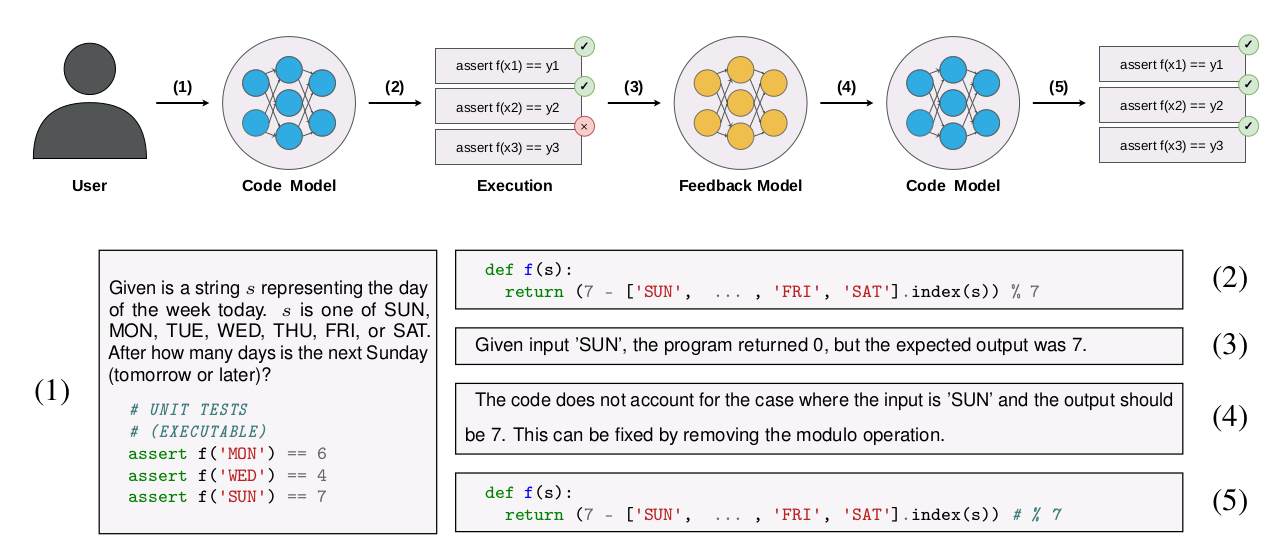
\includegraphics[scale=0.25]{png/example.png}
    \begin{itemize}
        \item 如上图所示,是一个代码任务的自我修复能力的展示,用户给定一个任务,然后返回一个代码,之后检测该代码是否有bug,有的话进行使用反馈模型进行修复,重新检测代码,直至没有问题再输出.
    \end{itemize}
\end{frame}

\begin{frame}
    \frametitle{模型使用的方法}
    \begin{itemize}
        \item 该论文提出了一种名为 pass @ t 的新评估策略,该策略根据从模型中采样的tokens总数来衡量任务的通过率,从而可以与纯粹基于采样的方法进行公平比较。
        \item 本文分析了 GPT-3.5 和 GPT-4 对包含各种编码挑战的具有挑战性的数据集进行自我修复的能力。 
        \item  这个的方法主要分为4个步骤,代码生成,代码执行,反馈生成,代码修复\\
        % \item 该论文将使用 GPT-4 进行自我修复的性能与 GPT-3.5 和专业人类程序员的反馈进行了比较。
    \end{itemize}
\end{frame}

\begin{frame}
    \frametitle{结论}
    \eee{
        \item GPT-3.5 无法对具有挑战性的编码任务进行自我修复。
        \item 尽管在 GPT-4 中可以看到绩效提升,但效果不大,依赖于在初始项目中实现足够的多样性。 
        % \item 用 GPT-4 改进的性能代替 GPT-3.5 的反馈,甚至超过了 GPT-3.5 的基线。 
        \item 用经验丰富的程序员提供的反馈取代 GPT-4 自行生成的反馈,使通过所有单元测试的修复程序数量增加了 57\%。
        % \item 该论文表明,使用 GPT-4 对 GPT-3.5 生成的程序提供反馈并使用专业的人类程序员对 GPT-4 生成的程序提供反馈可以显著提高性能。
    }
\end{frame}

% \subsection{MEGABYTE的新方法}
% \begin{frame}
%     \frametitle{这个模型需要}
% \end{frame}


\begin{frame}
    \frametitle{相关启示}
    \begin{itemize}
        \item 修改当前的评估指标,改成pass @ t的评估指标,使得比较更加的公平
    \end{itemize}

\end{frame}

% \subsection{论文2} 
% \begin{frame}
%     \frametitle{MEGABYTE的新方法}
%     \begin{itemize}
%         \item 摘要:该论文提出了一种名为MEGABYTE的新方法,用于对超过一百万字节的长序列进行建模。它使用多尺度解码器架构,将序列分成补丁,并在补丁中使用局部子模型,在补丁之间使用全局模型,从而实现次二次自我注意力,提高解码过程中的并行性。
%         \item 本文的贡献如下:
%         \eee{
%             \item 引入 MEGABYTE,这是一种使用多尺度解码器架构对长字节序列进行建模的新方法,该架构将序列分成补丁,在补丁中使用本地子模型,在补丁之间使用全局模型。en
%             \item 对 MEGABYTE 和强基线进行了广泛的实验,表明 MEGABYTE 允许字节级模型在长上下文语言建模中与子词模型竞争,在 ImageNet 上实现最先进的密度估计困惑,并允许从原始音频文件进行音频建模。n
%             \item 观察到,对于许多任务,大多数字节预测相对容易,这意味着没有必要按字节计算大型网络,并且可以使用小得多的模型进行补丁内建模。
%         }
%         \item introduction:该论文的介绍突显了音乐、图像或视频文件等各个领域中数百万字节的序列无处不在。但是,大型变压器解码器通常只使用数千个上下文令牌,这限制了可以应用它们的任务集。本文介绍了 MEGABYTE,这是一种使用多尺度解码器架构对长字节序列进行建模的新方法,该架构将序列分成补丁,在补丁中使用局部子模型,在补丁之间使用全局模型。这种方法可以实现亚二次的自我注意力,提高解码过程中的并行度,从而以更低的成本提高训练和生成性能。
%         \item method:该论文提出了一种名为MEGABYTE的新方法,该方法使用多尺度解码器架构对长字节序列进行建模,该架构将序列分成补丁,并在补丁中使用局部子模型,在补丁之间使用全局模型。这种方法可以实现亚二次的自我注意力,提高解码过程中的并行度,从而以更低的成本提高训练和生成性能。该论文还对MEGABYTE和强基线进行了广泛的实验,表明MEGABYTE允许字节级模型在长上下文语言建模中与子词模型竞争,在ImageNet上实现最先进的密度估计困惑,并允许从原始音频文件进行音频建模。此外,本文还讨论了使用语言模型在推理过程中用速度换取性能的几种技巧,包括滑动窗口和跨步推理。但是,这些方法仅在与先前发表的作品进行比较时使用。
%         \item result:该论文对MEGABYTE和强基线进行了广泛的实验,表明MEGABYTE允许字节级模型在长上下文语言建模中与子词模型竞争,在ImageNet上实现最先进的密度估计困惑,并允许从原始音频文件进行音频建模。本文还讨论了使用语言模型在推理过程中用速度换取性能的几种技巧,包括滑动窗口和跨步推理。但是,这些方法仅在与先前发表的作品进行比较时使用。
%         \item conclusion:该论文得出的结论是,拟议的多尺度解码器架构MEGABYTE是一种用于对长序列进行建模的可扩展方法,在一系列任务和模式中,它的性能优于现有的字节级模型,允许使用超过100万个令牌的大型序列。它还使用子词模型提供了具有竞争力的语言建模结果,这可能允许字节级模型取代标记化。但是,这里的实验规模远低于最先进的语言模型的规模,未来的工作应该探索将MEGABYTE扩展到更大的模型和数据集。
%     \end{itemize}
%     \eee{
%         \item 这个模型需要对transformer很了解才能看,还是就算了,不看这篇了.
%     }
% \end{frame}




% \subsection{论文3}
% \begin{frame}
%     \frametitle{大规模气象数据进行全面的天气预报}
%     \begin{itemize}
%         \item 摘要:论文摘要描述了需要一个协作平台,用于对大规模气象数据进行全面的天气预报。该论文提出了一种新颖的联邦学习方法,用于在具有异构气象数据的参与者中协作学习基于时空变压器的基础模型,以及一种满足资源匮乏传感器的通信和计算限制的即时学习机制。
%         \item 本文的贡献如下:
%         \eee{
%             \item 开发能够理解复杂的气象数据并提供跨区域天气预报的基础模型。 
%             \item 提出一种新颖的联邦学习方法,用于在具有异构气象数据的参与者中协作学习基于时空变压器的基础模型。 
%             \item 采用一种新颖的即时学习机制来满足资源匮乏传感器的通信和计算限制。 
%             \item 使用三个具有多变量时间序列的气象数据集,演示了拟议方法在经典天气预报任务中的有效性。
%         }
%         \item introduction:论文的导言强调了全球气候变化对不同区域的影响,以及需要一个大规模的协作数据共享平台来应对这一挑战。本文建议使用机器学习技术来提高解决这个问题的效率。但是,区域的异质性给采用集中统一模式为所有区域提供服务带来了挑战。
%         \item method:该论文提出了一种新颖的联邦学习方法,用于在具有异构气象数据的参与者中协作学习基于时空变压器的基础模型。所提出的方法使用一种新颖的即时学习机制来满足资源匮乏传感器的通信和计算限制。本文还介绍了一种空间即时学习(SPL)方法,该方法可以从空间角度在本地客户身上建立气象因素之间的相关性。使用三个具有多变量时间序列的气象数据集,证明了所提出的方法在经典天气预报任务中的有效性。
%         \item result:本文使用三个具有多变量时间序列的气象数据集,演示了所提出的方法在经典天气预报任务中的有效性。结果表明,所提出的方法在预测精度和效率方面优于最新方法。具体而言,所提出的方法显著提高了温度和降水的预测精度,而温度和降水是天气预报的关键因素。该论文还表明,该方法可以有效处理各地区气象数据的异质性,缓解数据暴露问题。
%         \item conclusion:该论文提出了一种新的机器学习方法来训练天气预报任务的基础模型,该方法能够捕捉基于多变量时间序列的气象数据的时空关系。本文在FL框架内引入了一种基于固定基础模型的即时学习机制,以提高性能,同时保持数据安全并减少通信开销。此外,该论文利用基于图的方法来减轻数据异质性对模型有效性的影响。使用三个具有多变量时间序列的气象数据集,证明了所提出的方法在经典天气预报任务中的有效性。本文得出结论,该方法在预测精度和效率方面优于最先进的方法,可以有效处理各地区气象数据的异质性,缓解数据暴露问题。
%     \end{itemize}
%     \eee{
%           \item 这篇文章意义也不是很大!!
% }
% \end{frame}



\section{代码调试}

\subsection{结果展示}

\begin{frame}
    \frametitle{\tiny 训练总数据量:30000;预测长度:16预测8;用于训练函数序列:\ff{[x,Cos(x),Sin(x^2+2),Sin(x)]}   \\
    待预测的数据:8预测4;预测的函数序列:\ff{[x,Cos(x),Sin(x^2+2),Sin(x)]};准确率:0\%}
	\begin{itemize}
		% \item 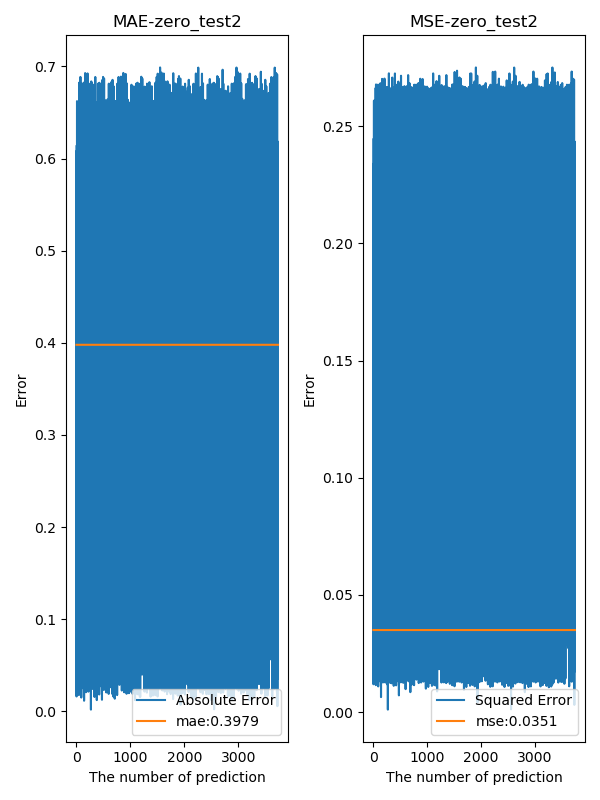
\includegraphics[scale=0.3555]{png/zero_test2.png}
        \item 最终预测的所有结果都是长度为8的,但对于单一的任务是没有泛化能力的.
	\end{itemize}
\end{frame}


\begin{frame}
	% \frametitle{\tiny 准确率:99.78\%,使用具有result-8-3-4的结果去预测result-8-3-1}
    \frametitle{\tiny 训练总数据量:30000,预测长度:16预测8,用于训练函数序列:\ff{[x,Cos(x),Sin(x^2+2),Sin(x)]}   \\
    待预测的数据:16预测8,预测的函数序列:\ff{[x,sin(x)]}, 准确率:99.78\%}
	\begin{itemize}
		\item 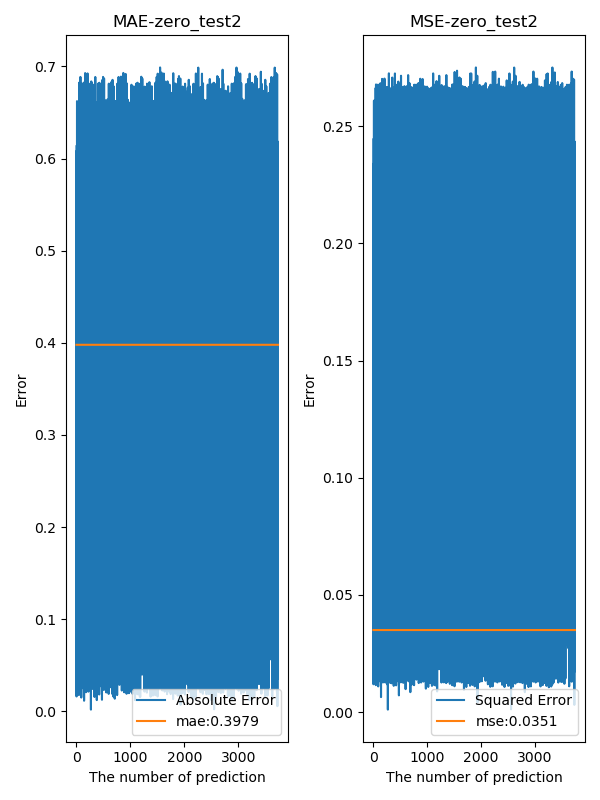
\includegraphics[scale=0.3555]{png/zero_test2.png}
		% \item 这个实验是对函数种类(简单对复杂)的泛化能力的测试,即能够预测[x,sin(x)]函数的模型,能否预测[x,Cos,tri\_poly,Sin]函数模型。
	\end{itemize}
\end{frame}


\begin{frame}
    \frametitle{\tiny 训练总数据量:30000,预测长度:16预测8,用于训练函数序列:\ff{[x,sin(x)]}   \\
    待预测的数据:16预测8,预测的函数序列:\ff{[x,Cos(x),Sin(x^2+2),Sin(x)]}, 准确率:99.97\%}    
    % \frametitle{\tiny 准确率:99.97\%,使用具有result-8-3-1的结果去预测result-8-3-4}
	\begin{itemize}
		\item 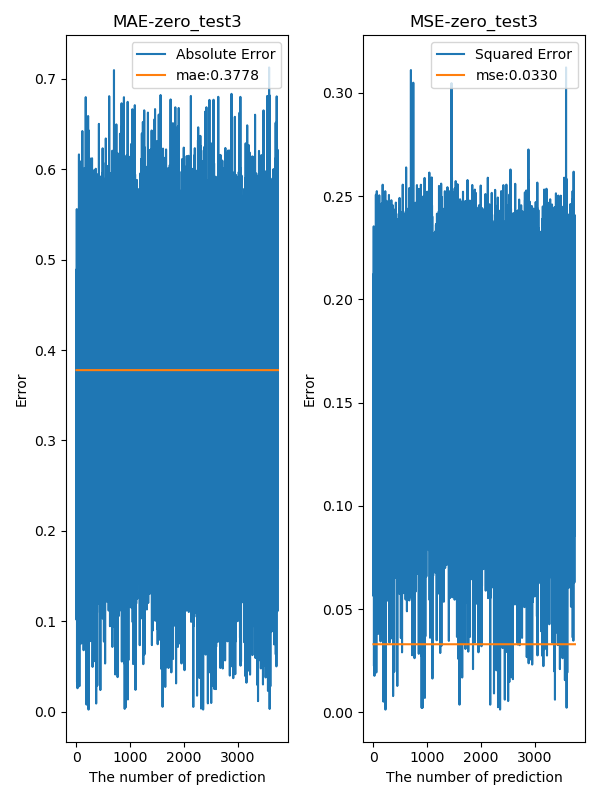
\includegraphics[scale=0.3555]{png/zero_test3.png}
		% \item 这个实验是对函数种类(复杂对简单)的泛化能力的测试,即能够预测函数[x,Cos,tri\_poly,Sin]的模型,能否预测[x,sin(x)]函数模型.
	\end{itemize}
\end{frame}

\begin{frame}
	% \frametitle{\tiny 准确率:37.11\%,使用具有mix\_5000\_8-18-2\_4-func的结果去预测mix\_5000\_16-80-4\_2-function}
    \frametitle{\tiny 训练总数据量:100000,预测长度:8预测4,...,18预测9,其中间隔为2;用于训练的函数序列:
    % \ff{[x,Sin],... }
    4种不同的函数序列;   \\
    待预测的数据:16预测8,...,80预测40,间隔为4;预测的函数序列:2种不同的函数序列;准确率:37.11\%}        
	\begin{itemize}
		\item 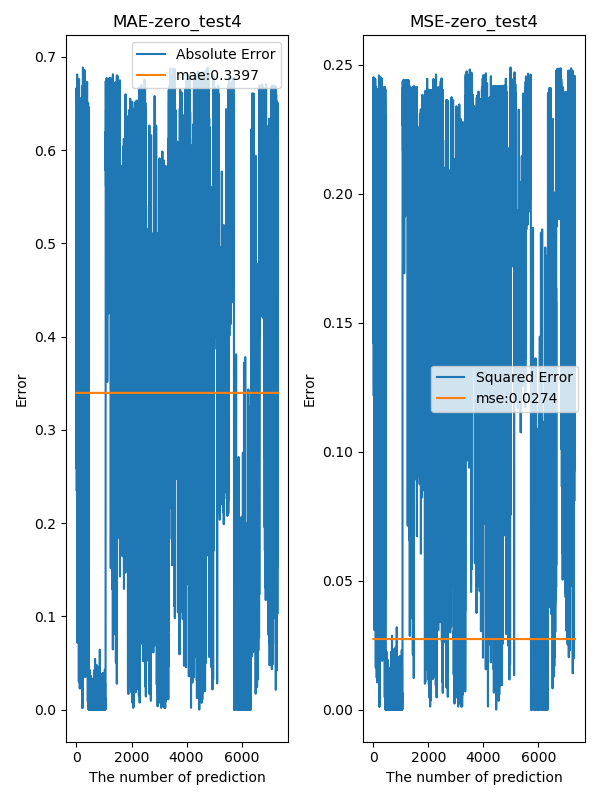
\includegraphics[scale=0.3555]{png/zero_test4.png}
		% \item 具有大型能力的模型之间的相互预测,目的是测试函数种类多,序列种类少这两种模型哪种泛化能力的效果更好。
	\end{itemize}
\end{frame}

\begin{frame}
	% \frametitle{\tiny 准确率:7.14\%,使用具有data\_large去预测mix\_5000\_16-80-4\_2-function中的内容}
    \frametitle{\tiny 训练总数据量:120000,预测长度:8预测4,16预测8;用于训练的函数序列:
    2种不同的函数序列;   \\
    待预测的数据:16预测8,...,80预测40,间隔为4;预测的函数序列:2种不同的函数序列(和训练的函数序列相同);准确率:7.14\%}
    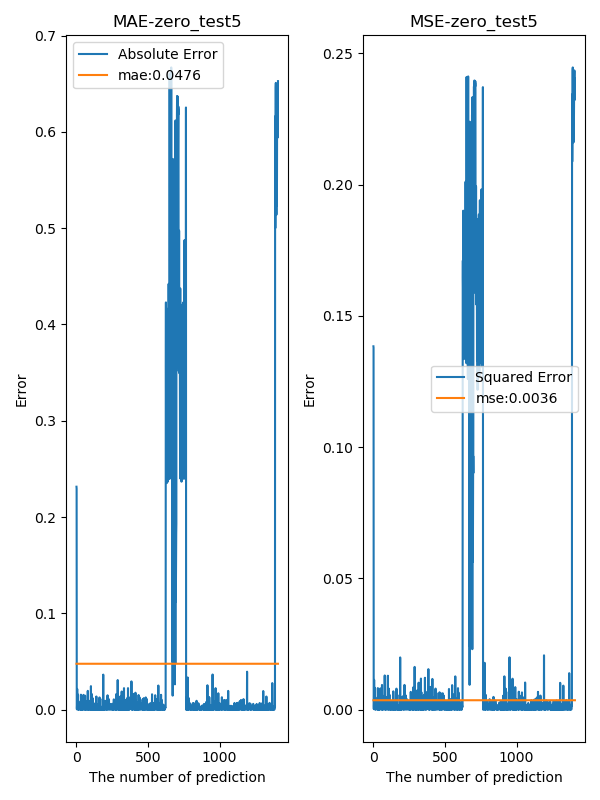
\includegraphics[scale=0.3555]{png/zero_test5.png}
	% \begin{itemize}
	% 	\item 
	% 	\item 目的是测试是否训练足够多的数量以后可以得到更好的泛化能力。
	% \end{itemize}
\end{frame}

\begin{frame}
	% \frametitle{\tiny 准确率:66.95\%,使用具有zero\_model\_test去预测mix\_5000\_16-80-4\_2-function中的内容}
    \frametitle{\tiny 训练总数据量:160000,预测长度:8预测4,...,24预测12,间隔4;用于训练的函数序列:4种不同函数序列 \\
    待预测的数据:16预测8,...,80预测40,间隔为4;预测的函数序列:2种不同的函数序列;准确率:99.48\%} 
    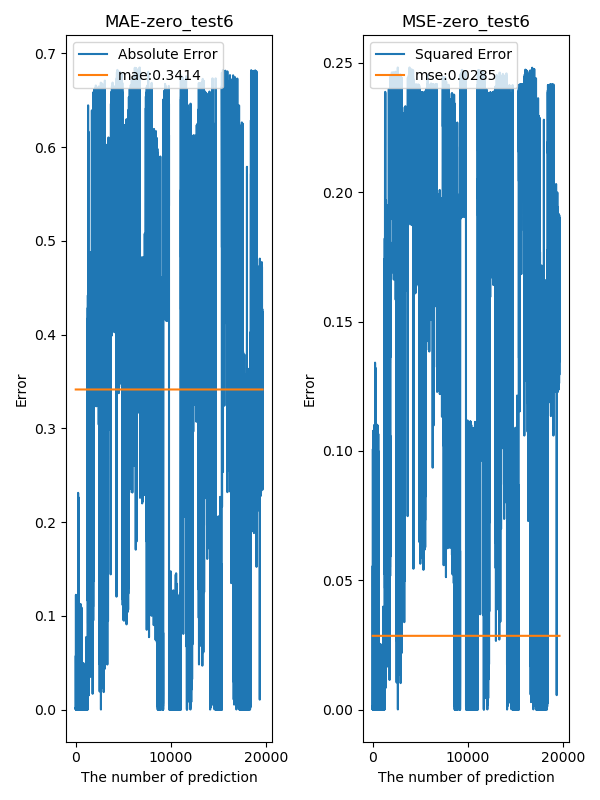
\includegraphics[scale=0.3555]{png/zero_test6.png}
	% \begin{itemize}
		%	\item 是否一个更加综合的模型能够对结果有更强的泛化能力?
	% \end{itemize}
\end{frame}


\begin{frame}
	% \frametitle{\tiny 准确率:66.95\%,使用具有zero\_model\_test去预测mix\_5000\_16-80-4\_2-function中的内容}
    \frametitle{\tiny 训练总数据量:640000,预测长度:8预测4,...,80预测40,间隔4;用于训练的函数序列:8种基本函数,如三角,多项式函数,对数,平方根等 \\
    待预测的数据:16预测8,...,80预测40,间隔为4;预测的函数序列:2种不同的函数序列;准确率:66.95\%} 
    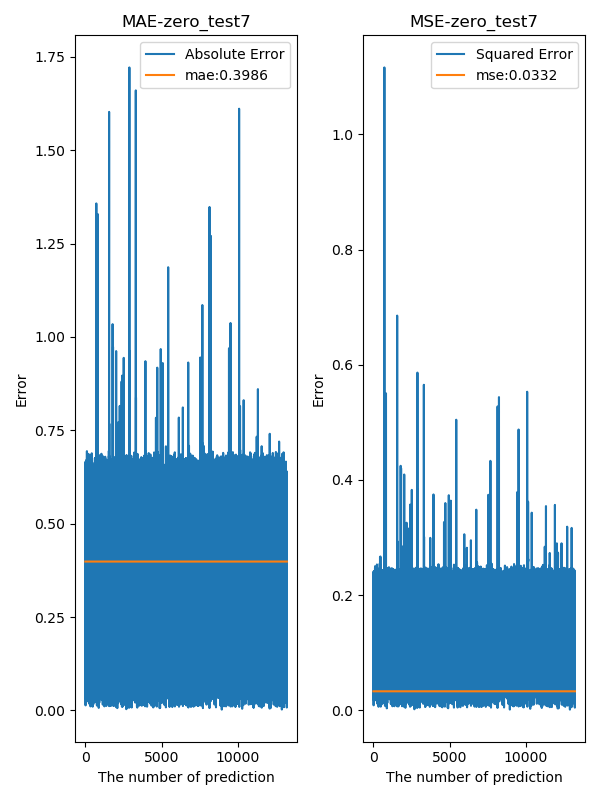
\includegraphics[scale=0.3555]{png/zero_test7.png}
	% \begin{itemize}
		%	\item 是否一个更加综合的模型能够对结果有更强的泛化能力?
	% \end{itemize}
\end{frame}


% \begin{frame}
% 	\frametitle{\small 总数据量:30000,16预测8,长向量序列预测}	
% 	\begin{itemize}
% 		% \item 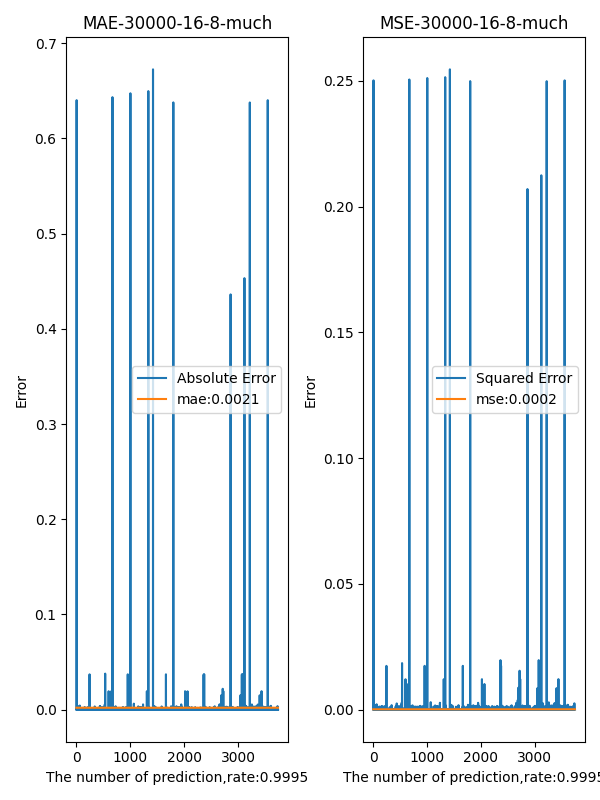
\includegraphics[scale=0.3555]{png/30000-16-8-much.png}
% 	\end{itemize}
% \end{frame}

\subsection{实验结果分析}
\begin{frame}
	\frametitle{实验结论}	
	\begin{itemize}
        \item 第一个实验中,预测的函数序列和训练的函数序列相同,但预测序列的长度和训练的长度不同,,结果发现正确的预测长度应该是4,但是结果预测长度全部是8.从中可以看出,模型对于解决预测长度不同的问题的能力较弱.
        \item 第二个实验中,训练的函数不同,但是预测和训练的长度都相同,准确率明显上升,从中可知
        \eee{
            \item 与第一个实验相比,想要模型有较高的准确率,需要和训练数据的长度尽可能的接近.
            \item 在没见过的函数序列预测上,相比预测同一个函数序列,误差明显变大.之前的实验中MAE是0.001
        }
        \item 第三个实验中,训练的函数不同,但是预测和训练的长度都相同,相比上一个实验中,这个实验测试的是维度更高的函数序列预测维度更低的函数序列是否有更高的精度.
        \eee{
            \item 
            \item 从结果的准确率和最终预测误差来看,使用更高维度来预测低维度和低维度预测高维度的基本差不多,所以函数维度大小对模型泛化性能影响不大.
        }        
	\end{itemize}
\end{frame}

\begin{frame}
    \frametitle{实验结论}
    \begin{itemize}
        \item 第四个实验中,训练和预测的序列长度和种类都不同.即去预测一个长度,函数序列都不同的序列,有如下的结论
        \eee{
            \item 准确率较低,预测结果的误差也比较大.并但是训练的模型更复杂,相比第一种实验中训练简单的模型,准确率上有明显的提升.
        }
        \item 第五个实验中,相比第四个实验中,将序列数量和函数种类都减少,再去预测相同的内容,最终的发现准确率更低了.
        \eee{
            \item 这说明训练时更复杂的数据集,能够让准确率提高.
            \item 预测结果误差由于样本少,不好判断
        }
        \item 第六个实验中,预测长度更接近和且更多种类的函数序列来进行预测,且将单种类型的数据量从之前实验的5000提高到10000.
        \eee{
            \item 从结果中可以看到,数据量提高且训练的序列长度和预测的长度更接近以后,最终的准确率会有显著提高.
            \item 预测结果的误差依旧没有明显的减小.
        }
    \end{itemize}    
\end{frame}

\begin{frame}
    \frametitle{实验结论}
    \begin{itemize}
        \item 第七个实验中,用了一个预测序列形式相同,但是函数序列种类更多的一个模型,对相同的数据进行预测.得到结果
        \eee{
            \item 从准确率中可以看到,当预测和训练的长度相同时,训练的函数序列种类变多反而导致最终的准确率下降了.
            \item 预测结果的误差也没有发生明显的变化.
        }
\end{itemize}
    
\end{frame}

% \subsection{实验过程中遇到的一些问题}

% \begin{frame}
% 	\frametitle{遇到的问题}	
% 	\begin{itemize}
%         \item 目标预测的个数和实际预测个数不同或者预测非数值形式,下面是一些解决方法
%         \eee{
%             \item 忽略实际预测个数和目标个数不同的例子,并计算其比率rate(目标与实际个数相同的个数/测试集个数)
%             \item 对预测得到的结果进行截断或补零
%         }   
%         \item 序列长度太长的问题
% 	\end{itemize}
%     % 目前考虑的是只考虑数量对等的
% \end{frame}


\subsection{下一步的计划}
\begin{frame}
	\frametitle{实现目标}	
	\begin{itemize}
        % \item 混合更多的元素,同时训练更多不同种类的时间序列和以及预测长度。
        % \item 尝试对未见过的序列进行预测,看看结果如何。
        \item 修改提示方式,比如表示数字的时候用\$符号等方式。
        \item 如何提高模型的泛化能力,在准确率上可以让训练的模型尽可能的进行多种不同长度序列的测试.在预测结果的误差上,还不太清楚如何减小误差.
        % \item 使用别的chatglm2尝试一下吧
        \item 现在最大的问题就是,如何能够改善模型的泛化能力,特别是在预测结果误差上的改进.
        % \item 尝试使用其中一篇文章中的MEGABYTE方法来处理长序列进行建模,以解决时间数据集中序列过长的问题。
        % \item 对于结果多次试验,取平均
        % \item 提高模型参数精度,看看结果是否会有什么变化。        
        % \item 开始对8个常见的时间序列进行测试。
	\end{itemize}
\end{frame}

% \subsection{图像结果展示}
% \subsection{测试的数据集}


% \section{相关论文}
% \begin{frame}
%     \frametitle{prompt learning and time series论文(IEEE)}
% \eee{
%     \item 标题:Evaluating BERT on cloud-edge time series forecasting and sentiment analysis via prompt learning\\
%     \item 结论:该论文使用即时学习评估了在云边缘时间序列预测和情感分析任务的大量数据上预训练的BERT的性能。实验结果表明,BERT在云边时间序列预测任务中表现不佳,这表明BERT没有良好的逻辑推理能力。选择均方误差 (MSE) 作为时间序列预测的评估指标,结果表明,使用即时学习的 BERT 无法根据前一个滑动窗口中的信息很好地预测下一个时间步长的特征。
% }    
% \end{frame}


% 结束语
\section{}
\begin{frame}
	\frametitle{}
	\begin{center}
		\Huge{谢谢老师和同学的聆听!}
	\end{center}
\end{frame}

\end{CJK*}
\end{document}